% ^^A documentation part start with %
% ^^A All other parts are called definition parts
% ^^A Comments in documentation part
% ^^A equivalently use \iffalse ... \fi
% \iffalse meta-comment
% !TeX program = XeLaTeX
% !TeX encoding = UTF-8
%
% Copyright (C) 2016 by Van Abel <van141.abel(AT)gmail.com>
% ---------------------------------------------------------------------
%
% This work may be distributed and/or modified under the
% conditions of the LaTeX Project Public License, either
% version 1.3c of this license or (at your option) any later
% version. This version of this license is in
%    http://www.latex-project.org/lppl/lppl-1-3c.txt
% and the latest version of this license is in
%    http://www.latex-project.org/lppl.txt
% and version 1.3 or later is part of all distributions of
% LaTeX version 2005/12/01 or later.
%
% This work has the LPPL maintenance status `maintained'.
%
% The Current Maintainers of this work is Van Abel.
%
% ---------------------------------------------------------------------
%
%<*internal>
\iffalse
%</internal>
%<*readme>
---------------------------------------------------------------
mathexam --- A package for math exam
===============================================================
Released under the LaTeX Project Public License v1.3c or later
See http://www.latex-project.org/lppl.txt
---------------------------------------------------------------
This package is developed when I prepare the midterm exam in the Shanghai Jiao Tong University. It based on the `multicol` package to create two column typesetting, and `eso-pic` package to add the basic infomation, such as the title, the score table, as a background image.

USAGE
---------------------------------------------------------------
Download the zip file and unzip to a local directory, then have a look at the `mathexam-main.pdf`, you can edit and compile it by `latexmk -xelatex -shell-escape mathexam-main.tex`.
%</readme>
%<*internal>
\fi
\def\nameoflatex{plain}
\ifx\nameoflatex\fmtname\else
  \expandafter\begingroup
\fi
%</internal>
%
%<*install>

\input docstrip.tex
\keepsilent
\askforoverwritefalse
\preamble
----------------------------------------------------------------
mathexam --- A package for math exam
===============================================================
E-mail: van141.abel(AT)gmail.com
Released under the LaTeX Project Public License v1.3c or later
See http://www.latex-project.org/lppl.txt
----------------------------------------------------------------

\endpreamble
\postamble

Copyright (C) 2009 by You <van141.abel(AT)gmail.com>

This work may be distributed and/or modified under the
conditions of the LaTeX Project Public License (LPPL), either
version 1.3c of this license or (at your option) any later
version.  The latest version of this license is in the file:

http://www.latex-project.org/lppl.txt

This work is "maintained" (as per LPPL maintenance status) by
You.

This work consists of the file  mathexam.dtx
and the derived files           mathexam.ins,
                                mathexam-main.tex,
                                mathexam-main.pdf,
                                mathexam.pdf and
                                mathexam.sty.

\endpostamble
\generate{
  \usedir{tex/latex/mathexam}
  \file{\jobname.sty}{\from{\jobname.dtx}{package}}
  \nopreamble\nopostamble
  \file{\jobname-main.tex}{\from{\jobname.dtx}{maintex}}
  \usedir{doc/latex/mathexam}
  \file{README.txt}{\from{\jobname.dtx}{readme}}
}
\obeyspaces
\Msg{****************************************************}
\Msg{*                                                   }
\Msg{* To finish the installation you have to move the   }
\Msg{* following file into a directory searched by TeX   }
\Msg{* e.g. tex/latex/mathexam:                          }
\Msg{*                                                   }
\Msg{* \jobname.sty                                      }
\Msg{*                                                   }
\Msg{* To produce the documentation run the file         }
\Msg{* \jobname.dtx through XeLaTeX.                     }
\Msg{*                                                   }
\Msg{* To produce the sample file run the file           }
\Msg{* \jobname-main.tex through XeLaTeX and BibTeX      }
\Msg{*                                                   }
\Msg{* Happy TeXing!                                     }
\Msg{*                                                   }
\Msg{****************************************************}
%</install>
%<install>\endbatchfile
%
%<*internal>
  \usedir{source/latex/mathexam}
  \generate{
    \file{\jobname.ins}{\from{\jobname.dtx}{install}}
  }
% ^^A No extra text add by DocStrip
  \nopreamble\nopostamble
  \usedir{doc/latex/ustcmb}
  \generate{
    \file{README.md}{\from{\jobname.dtx}{readme}}
  }
% ^^A if xetex then end process of DocStrip by \endbatchfile
\ifx\nameoflatex\fmtname
  \expandafter\endbatchfile
\else
% ^^A for xelatex we close the group
  \expandafter\endgroup
\fi
%</internal>
%
%<*driver>
\ProvidesFile{\jobname.dtx}
%</driver>
%<package>\NeedsTeXFormat{LaTeX2e}[2005/12/01]
%<package>\ProvidesPackage{mathexamp}
%<*package>
[2018/12/23 v.1.0.0 A package for math exam]
%</package>
%
%<*driver>
\documentclass{ltxdoc}
\usepackage{palatino}
\usepackage{ctex}
\usepackage[margin=1in, includeheadfoot]{geometry}
\usepackage[numbered]{hypdoc}

\EnableCrossrefs
\renewcommand\indexname{Index}
\IndexPrologue{%
  \section*{\indexname}
  \textit{Numbers written in italic refer to the page where the corresponding entry is described; numbers underlined refer to the definition; numbers in roman refer to the
pages where the entry is used.}
}
\CodelineIndex
\RecordChanges
\def\glossaryname{Version History}
\GlossaryPrologue{\section*{\glossaryname}}
\begin{document}
  \DocInput{\jobname.dtx}
  \PrintChanges
  \PrintIndex
\end{document}
%</driver>
% \fi
%
% \CharacterTable
%  {Upper-case    \A\B\C\D\E\F\G\H\I\J\K\L\M\N\O\P\Q\R\S\T\U\V\W\X\Y\Z
%   Lower-case    \a\b\c\d\e\f\g\h\i\j\k\l\m\n\o\p\q\r\s\t\u\v\w\x\y\z
%   Digits        \0\1\2\3\4\5\6\7\8\9
%   Exclamation   \!     Double quote  \"     Hash (number) \#
%   Dollar        \$     Percent       \%     Ampersand     \&
%   Acute accent  \'     Left paren    \(     Right paren   \)
%   Asterisk      \*     Plus          \+     Comma         \,
%   Minus         \-     Point         \.     Solidus       \/
%   Colon         \:     Semicolon     \;     Less than     \<
%   Equals        \=     Greater than  \>     Question mark \?
%   Commercial at \@     Left bracket  \[     Backslash     \\
%   Right bracket \]     Circumflex    \^     Underscore    \_
%   Grave accent  \`     Left brace    \{     Vertical bar  \|
%   Right brace   \}     Tilde         \~}
%
%\GetFileInfo{\jobname.dtx}
%
% \DoNotIndex{\%,\#,\$,\%,\&,\\,\^,\_,\~,\[,\],\',\`,\documentclass}
% \DoNotIndex{\@ne,\and,\author,\centerline,\date,\inst,\institute}
% \DoNotIndex{\AddToShipoutPictureBG, \ansbox, \ansheight}
% \DoNotIndex{\AtEndOfPackage, \captionof, \cdot, \cdots, \cfoot}
% \DoNotIndex{\columnsep, \columnwidth, \cos, \cosh, , \arctanh}
% \DoNotIndex{\definecolor,\decumentclass,\label,\newtheorem,\sc}
% \DoNotIndex{\fancyhf, \fill, \fontsize, \footrulewidth, \frac}
% \DoNotIndex{\arraystretch, \left\{,\right\}, \DeclareMathOperator}
% \DoNotIndex{\Delta, \delta, \draw, \emph, \endEnvironenv, \envbody}
% \DoNotIndex{\environbodyname, \Environenv, \eqref, \eta, \dotfill}
% \DoNotIndex{\exam@lasttwoofyear, \exam@showansfalse, \exam@showanstrue}
% \DoNotIndex{\exam@value@AorB, \exam@getlasttwo, \exam@value@coursename}
% \DoNotIndex{\exam@value@semester, \exam@value@univname, \expandafter}
% \DoNotIndex{\extracolsep, \linewidth, \ln, \lvert, \rvert, \qquad, \quad}
% \DoNotIndex{\makebox, \mathbb, \mathring, \month, \mycolsep, \gamma}
% \DoNotIndex{\getrefbykeydefault, \headrulewidth, \hspace, \ifexam@showans}
% \DoNotIndex{\ifnum, \ifdim, \iiint, \iint, \implies, \in, \infty, \int}
% \DoNotIndex{\lambda, \ldots, \left, \right, \leq, \lim, \limits}
% \DoNotIndex{\nabla, \NeedsTeXFormat, \newbox, \NewDocumentEnvironment}
% \DoNotIndex{\NewEnviron, \newlength, \null, \number, \numexpr, \Omega}
% \DoNotIndex{\PakcageWarning, \pagestyle, \parbox, \partial, \pi, \pm}
% \DoNotIndex{\ProvidesPackage, \ref, \savebox, \sech, \secondheader}
% \DoNotIndex{\selectfont, \settoheight, \settowidth, \Sigma, \sin, \sinh}
% \DoNotIndex{\sqrt, \setcounter, \subset, \substack, \sum, \tag, \tanh}
% \DoNotIndex{\the, \thecolumn, \thesection, \Theta, \theta, \thetotalcolumn}
% \DoNotIndex{\times, \titleformat, \to, \underline, \usebox, \usetikzlibrary}
% \DoNotIndex{\vec, \width, \xi, \year, \zhnum}
% \DoNotIndex{\setbeamercolor,\setbeamercovered,\setbeamertemplate}
% \DoNotIndex{\cite,\uwave,\cline,\eps,\epsilon,\geq}
% \DoNotIndex{\hline,\href,\item,\jobname,\lipsum,\lstinline}
% \DoNotIndex{\lstset,\small,\subsection,\textwidth,\ttfamily}
% \DoNotIndex{\tableofcontents, \setCJKmainfont,\setbeamerfont}
% \DoNotIndex{\setCJKmonofont,\setCJKsansfont,\subject,\subtitle}
% \DoNotIndex{\theoremstyle, \title, \titlepage, \usepackage}
% \DoNotIndex{\advance,\begingroup,\catcode,\closein}
% \DoNotIndex{\closeout,\day,\def,\edef,\else,\empty,\endgroup}
% \DoNotIndex{\addtobeamertemplate, \addtocounter}
% \DoNotIndex{\AtBeginDocument,\AtEndDocument,\AtEndOfClass}
% \DoNotIndex{\begin,\end,\bfseries,\bibliography}
% \DoNotIndex{\color,\CurrentOption,\DeclareOption,\fi,\frame}
% \DoNotIndex{\hfill,\hypersetup,\iftoggle,\includegraphics,\input}
% \DoNotIndex{\insertframenumber,\inserttotalframenumber}
% \DoNotIndex{\mode,\LARGE,\LoadClass,\necounter,\noewif,\nocite}
% \DoNotIndex{\numberwithin,\PassOptionsToClass,\pgfpagesuselayout}
% \DoNotIndex{\ProcessOptions, \providetoggle,\relax,\renewcommand}
% \DoNotIndex{\RequirePackage, \section, \setcounter, \toggletrue}
% \DoNotIndex{\value,\newcommand,\newif,\newcounter}
% \DoNotIndex{\ccwd,\caption,\captionsetup,\chapter,\ctexset}
% \DoNotIndex{\itemsep,\hangindent,\setfontsize,\setlength,\hdclindex}
% \DoNotIndex{\textbf,\newenvironment,\newcommand}
% \DoNotIndex{\n,\newCJKfontfamily,\AtBeginSubsection}
% \expandafter\DoNotIndex\expandafter{\string\&}
% \expandafter\DoNotIndex\expandafter{\string\{}
% \expandafter\DoNotIndex\expandafter{\string\}}
%\title{^^A
%  \textsf{mathexam} --- A package for math exam\thanks{^^A
%    This file describes version \fileversion, last revised \filedate.^^A
%  }^^A
%}
%\author{^^A
%  Van Abel\thanks{E-mail: van141.abel(AT)gmail.com}^^A
%}
%\date{Released \filedate}
%
%\maketitle
%\def\abstractname{Abstract}
%\begin{abstract}
%This is a package for preparing of typesetting math exam. It is developed when I prepare the midterm exam in the Shanghai Jiao Tong University. It based on the \verb|multicol| package to create two column typesetting, and \verb|eso-pic| package to add the basic infomation, such as the title, the score table, as a background image.
%\end{abstract}
%\changes{v1.0.0}{2018/11/23}{Initial version}
%
%\section{A short introduction for usage}
% Basically, to use the package |mathexam|, you only need to download the |mathexam.sty| and include it in your document by |\usepackage{mathexam}|. You can refer the example doc given in |mathexam-main.tex|. All the above mentioned files can be download at the release page as a zip compressed archive.
%
% To see the final typesetting, you can have a look at the |mathexam-main.pdf|.
%\section{Options, commands and environments}
%\subsection{Options}
%\DescribeMacro{showans}
% The option |showans| is a switch, without it the typeset will not show the answer.
%\subsection{Commands}
%\DescribeMacro{\univname}
% The command \cs{univname} is used to set the university name, which
% has a mandatory argument \marg{university name}.
%
%\DescribeMacro{\coursename}
% The command \cs{coursename} is used to set the course name, which
% has a mandatory argument \marg{course name}.
%
%\DescribeMacro{\AorB}
% The command \cs{AorB} is used to set the type of exam eithor A or B, which
% has a mandatory argument, the value is either \marg{A} or \marg{B}.
%
%\DescribeMacro{\scqt}
% The command \cs{scqt} is used to typeset the \emph{signle choice question}, which
% has a mandatory argument \marg{the title of the question}, and an optional argument,
% which is either \oarg{A}, \oarg{B}, \oarg{C} or \oarg{D}.
%
%\DescribeMacro{\scq}
% The command \cs{scq} is used to typeset the four choices of the \emph{signle choice question}, which has four mandatory arguments, they are the four choices of the question respectively. It also has an optional argument, which will type set the four choices in one line or two (this is not work in current version).
%
%\DescribeMacro{\fb}
% The command \cs{fb} is used to typeset the \emph{fill blank} items in the exam, which has two mandatory arguments, the first one is stands for the title of fill blank, and the last one is for the correct answer. It also has an optional argument, which typeset the width of the underline, the default is \meta{6em}.
%
%\subsection{Environments}
%\DescribeEnv{ans}
% The environment |ans| is used for typeset the answer of items which needs a long and detail calculation, argument or proof. It has two optional argument, the first one is for the title of the answer, the default is \emph{Solution}, and the second one is for add extra spaces after the answer, the default is \meta{2em}
%
%\StopEventually{}
%
%\section{Source code implementation}
%    \begin{macrocode}
%<*package>
\NeedsTeXFormat{LaTeX2e}[1996/06/01]
\ProvidesPackage{mathexam}[2018/12/23 v1.0.0 A package for math exam]
\RequirePackage{multicol}
\RequirePackage{mathtools, amssymb}
\RequirePackage{subfig}
\RequirePackage{eso-pic}
\RequirePackage{lipsum}
\RequirePackage{verbatim}
\RequirePackage{ctex}
\RequirePackage[
  a3paper,
  landscape,
  margin=2cm,
  includeheadfoot,
  headheight=0pt
]{geometry}
\RequirePackage{multido, ifthen} 
\RequirePackage{lastpage, refcount, fancyhdr}

\RequirePackage{calc}
\RequirePackage{tikzpagenodes}
\usetikzlibrary{calc}
\RequirePackage{zhnumber}
\renewcommand\thesection{\zhnum{section}、\hspace{-1em}}
\RequirePackage{titlesec}
\titleformat{\section}{\fontsize{14}{17}\selectfont\bfseries}{\thesection}{1em}{}

\newif\ifexam@showans\exam@showansfalse
\DeclareOption{showans}{
  \exam@showanstrue
}

\DeclareOption*{\PackageWarning{examplepackage}{Unknown ‘\CurrentOption’}}
\ProcessOptions\relax

\AddToShipoutPictureBG{% Add background picture to every page/ *version for current page
  \begin{tikzpicture}[overlay,remember picture]
    \draw [line width=1pt ]
      ($(current page text area.north west) +0.5*(-\mycolsep,\mycolsep)$)
      rectangle
      ($(current page text area.south east) +0.5*(\mycolsep,-\mycolsep)$);
    \draw [ dotted, line width=0.5pt ]
      ($(current page text area.north)+(0,0.5\mycolsep)$)
      --
      ($(current page text area.south)-(0,0.5\mycolsep)$);
 \end{tikzpicture}
}

\RequirePackage{xparse, environ}
\AtEndOfPackage{
  \newlength\mycolsep
  \setlength{\mycolsep}{1cm}
  \setlength{\columnsep}{\mycolsep}
  \renewcommand{\arraystretch}{1.2}
}


\newcommand{\scqt}[2][\qquad]{%
#2\hfill(\makebox[2em]{\ifexam@showans #1\fi})\\[1em]
}

\newcommand{\scq}[5][1]{%
  \makebox[0.25\linewidth][l]{(A) #2;}%
  \makebox[0.25\linewidth][l]{(B) #3;}%
  \makebox[0.25\linewidth][l]{(C) #4;}%
  \makebox[0.25\linewidth][l]{(D) #5.}%
}
\newcommand{\funderline}[2][2em]{%
\underline{\makebox[\ifdim\width>#1\width\else#1\fi]{#2}}%
}
\newlength\fbwidth
\newcommand{\fb}[3][6em]{%
  \settowidth{\fbwidth}{#3}
#2\funderline[\ifdim\fbwidth>#1\fbwidth\else#1\fi]{\ifexam@showans #3 \fi}.
}
\newlength\ansheight
\newcounter{cnt}
\newcommand{\ansskip}[1]{
  \setcounter{cnt}{0}
  \whiledo {\value{cnt} <100}
  {
    \vspace*{.01#1}\goodbreak
    \stepcounter{cnt}
  }
}
\NewDocumentEnvironment{ans}{O{答} O{2em}}
{\Environenv{
  \textbf{#1}:~}{#2}
}
{\endEnvironenv}
\newbox{\ansbox}
\environbodyname\envbody
\NewEnviron{Environenv}[2]{%
  \savebox{\ansbox}{
    \parbox[b]{\linewidth}{
      #1\envbody
    }
  }
  \settoheight{\ansheight}{\usebox\ansbox}
  \ifexam@showans
    \par#1\envbody
  \else
  \addtolength{\ansheight}{#2}
    \ansskip{\ansheight}
  \fi
}
\newcommand{\univname}[1]{\def\exam@value@univname{#1}}
\newcommand{\coursename}[1]{\def\exam@value@coursename{#1}}
\newcommand{\AorB}[1]{\def\exam@value@AorB{#1}}
\newcommand{\exam@value@semester}{\ifnum\the\month<9\ifnum\the\month>2 二\fi\else 一\fi}
\newcommand{\exam@lasttwoofyear}[1]{% #1 is the offset
  \expandafter\exam@getlasttwo\number\numexpr\year+(#1)\relax\relax
}
\def\exam@getlasttwo#1#2#3#4\relax{#3#4}
  \AtBeginDocument{
    \begin{multicols*}{2}
      \begin{center}
        {\fontsize{18}{22}\selectfont \textbf{
            \exam@value@univname(\funderline{\exam@value@AorB}卷)
          }
        }\\[0.5em]
        {\selectfont  20\funderline{\exam@lasttwoofyear{0}} 至20
        \funderline{\exam@lasttwoofyear{1}} 学年\qquad 第
        \funderline{\exam@value@semester}学期}
      \end{center}
      班级号\funderline[0.5\linewidth-8em]{}\qquad
      学号\funderline[0.5\linewidth-8em]{}\qquad
      姓名\funderline[5em]{} \\[0.5em]
      课程名称\funderline[\linewidth-13em]{\exam@value@coursename}\qquad
      成绩\funderline[5em]{ }
    }
    \AtEndDocument{
    \end{multicols*}
  }
  \newcommand{\secondheader}{
    \begin{minipage}[b]{0.18\columnwidth}
      \textbf{我承诺, 我将严格遵守考试纪律.}\\[1em]
      \textbf{承诺人}:\funderline[4em]{ }
    \end{minipage}\hfill
    \begin{minipage}[b][][t]{0.8\columnwidth}
      \begin{tabular*}{\linewidth}{@{\extracolsep{\fill} } |p{7em}|c|c|c|c|c|c|c|c|c|c|}
        \hline
        题号&一&二&三&四&五&六&七&八&九&十\\
        \hline
        得分&&&&&&&&&&\\
        \hline
        评阅人(流水阅
        卷教师签名处)&&&&&&&&&&\\
        \hline
      \end{tabular*}
    \end{minipage}
  }

\AtBeginDocument{
\pagestyle{fancy}
\fancyhf{}
\renewcommand{\headrulewidth}{0pt}
\renewcommand{\footrulewidth}{0pt}
\newcounter{column}
\newcounter{totalcolumn}
\setcounter{totalcolumn}{2*\getrefbykeydefault{LastPage}{page}{1}}
	\cfoot{
		\makebox[\columnwidth]{
			\stepcounter{column}%
			\funderline{\exam@value@AorB}卷\quad%
			共 \funderline{\thetotalcolumn}页, 第\funderline{\thecolumn}页%
			\hspace{\columnsep}%
		}%
		\makebox[\columnwidth]{
			\stepcounter{column}%
			\funderline{\exam@value@AorB}卷\quad%
			共 \funderline{\thetotalcolumn}页, 第\funderline{\thecolumn}页%
			\hspace{\columnsep}%
		}%
	}
}
%</package>
%<*maintex>
\documentclass[cs4size]{article}
\usepackage[showans]{mathexam} %showans

\univname{上海交通大学}
\coursename{高等数学(A)(2)}
\AorB{A}

\DeclareMathOperator{\sech}{sech}
\DeclareMathOperator{\arctanh}{arctanh}
\begin{document}
  \section{单项选择题(每小题3分, 共15分)}
  \begin{enumerate}
    \item \scqt[B]{函数$f(x,y)=\sqrt{x^2+y^2}$在$(0,0)$处}
      \scq{不连续}{连续但不可偏导}{可偏导但不可微}{可微}
    \item \scqt[A]{$f(x,y)=\sqrt{(x-1)^2+y^2}$在约束条件$2x+y-1=0$下的最小值为:}
      \scq{$\frac{1}{\sqrt{5}}$}{$\frac{2}{\sqrt{5}}$}{1}{2}
    \item \scqt[C]{圆盘$D:x^2+y^2\leq2^2$上的二重积分$\iint_D\sqrt{4-x^2-y^2}dxdy$等于}
      \scq{$16\pi$}{$8\pi$}{$\frac{16\pi}{3}$}{$\frac{8\pi}{3}$}
    \item \scqt[B]{椭球$\Omega=\left\{ (x,y,z): \frac{x^2}{a^2}+\frac{y^2}{b^2}+
      \frac{z^2}{c^2}\leq1 \right\}$上的三重积分$\iiint_\Omega\sqrt{1- \frac{x^2}{a^2}-
      \frac{y^2}{b^2}-\frac{z^2}{c^2}}dV$等于}
      \scq{$\frac{\pi^2}{4}$}{$\frac{\pi^2abc}{4}$}{$\pi^2$}{$\pi^2abc$}
    \item \scqt[C]{假设$\gamma$为曲面$x^2+y^2+z^2=1$与平面$y=x$的交线.
      曲线积分$\int_\gamma\sqrt{2y^2+z^2}ds$等于}
      \scq{$0$}{$\pi$}{$2\pi$}{$\pi/2$}
  \end{enumerate}
  \section{填空题(每小题3分, 共15分)}
  \begin{enumerate}\addtocounter{enumi}{5}
    \item \fb{假设$f(u)$是连续函数. 若$F(t)=\iiint_{x^2+y^2+z^2\leq t^4}
      f(x^2+y^2+z^2)dxdydz$, 则$F'(1)=$}{$8\pi f(1)$}
    \item \fb{假设函数$z=z(x,y)$的图像是以原点为心的上半球面.
      试求$z$在点$P(1,1,1)$处沿着方向$\vec{l}=(1,1)$的方向导数$=$}{-2}
    \item \fb{求$n$元径向对称函数$f(x_1,\ldots,x_n)=f(r)$的拉普拉斯
      $\Delta f=\sum_{i=1}^n \frac{\partial^2 f}{\partial x_i^2}$
      在极坐标下的表达示$=$}{$f''(r)+(n-1)f'(r)/r$}
    \item \fb{假设$z=f(x,y)$在点$P(1,1)$处连续.
      若$\lim\limits_{\substack{x\to1\\y\to1}}
      \frac{f(x,y)-x-2y+3}{\ln(1+(x-1)^2+(y-1)^2)}=\pi$,
      则全微分$dz|_{(1,1)}=$}{dx+2dy}
    \item \fb{求椭圆抛物面$z=2x^2+3y^2-1$与平面$4x+6y+z-1=0$平行的切平面方程}{4x+6y+z+6=0}
  \end{enumerate}
  \columnbreak
  \secondheader
\section{概念题(每小题5分, 共10分)}
\begin{enumerate}\addtocounter{enumi}{10}
  \item 假设二元函数$f(x,y)$在开区域
    $\Omega \subset \mathbb{R}^2$上有定义且在$P_0\in\Omega$处可微.
    试用$\epsilon$-$\delta$语言严格叙述: 在$P_0(0,0)\in \Omega$处$f$的全微分为$df(P_0)$.

    \begin{ans}[答][6em]
      即叙述存在常数$a,b\in \mathbb{R}$, 使得$df(P_0)=adx+bdy$. \dotfill{(1分)}\\
      用$\epsilon$-$\delta$语言叙述如下:
      对任意的$\epsilon>0$, 存在常数$\delta>0$, 使得对任意的
      $(x,y)\in \mathring{U}(P_0,\delta)$,
      即$0<\sqrt{x^2+y^2}\leq \delta$,\dotfill{(3分)}\\
      都存在常数$a,b\in \mathbb{R}$, 使得:
      \[
        \left\lvert \frac{f(x,y)-f(0,0)-ax-by}{\sqrt{x^2+y^2}} \right\rvert\leq\epsilon.\tag{5分}
      \]
    \end{ans}
  \item 假设二元函数$f=f(x,y)$, $g=g(x,y)$在有界闭区域$\Omega$上有定义.
    试严格写出关于$f$, $g$的积分中值定理.

    \begin{ans}
      二元函数的积分中值定理严格叙述如下:\\
      假设$f=f(x,y)$是有界闭区域$\Omega$上的连续函数,\dotfill{(1分)}\\
      $g=g(x,y)$是$\Omega$上的可积函数.\dotfill{(2分)}\\
      若$g$在$\Omega$上不变号\dotfill{(3分)}\\
      则存在$(\xi,\eta)\in \Omega$, 使得
      \[
        \iint_\Omega f(x,y)g(x,y)dxdy=f(\xi,\eta)\iint_\Omega g(x,y)dxdy.
        \tag{5分}
      \]
    \end{ans}
\end{enumerate}
\clearpage
\section{计算题(请写清楚计算的主要步骤. 每小题10分, 共20分)}
\begin{enumerate}\addtocounter{enumi}{12}
  \item 求锥面$z^2=x^2+y^2$被柱面$x^2+y^2=4x$割下部分曲面的表面积.
    \begin{ans}[解]
      由图易见, 被截部分是上下两个等表面积的曲面.
      为了参数化上半曲面, 我们注意到它在$Oxy$平面的投影为$(x-2)^2+y^2\leq 2^2$,
      故将上半曲面参数化为$(x,y,z=\sqrt{x^2+y^2})$,
      $(x,y)\in D=\left\{ (x,y):(x-2)^2+y^2\leq2^2 \right\}$. \dotfill{(2分)}

      注意到此时
      \[
        dS=\sqrt{1+z_x^2+z_y^2}=\sqrt{2}dxdy,\tag{5分}
      \]
      因此, 所求的表面积为
      \begin{align}
        I&=2\iint_D \sqrt{2}dxdy\tag{8分}\\
         &=2\sqrt{2}\cdot \pi 2^2=8\sqrt{2}\pi. \tag{10分}
      \end{align}
      \end{ans}
    \end{enumerate}
    %\vfill\null
    %\columnbreak
    \begin{enumerate}\addtocounter{enumi}{13}
      \item 假设$\Sigma$为椭球面$ \frac{x^2}{a^2}+\frac{y^2}{b^2}+\frac{z^2}{c^2}=1$
        的外侧, 计算积分$I=\iint_\Sigma zdxdy$.

        \begin{ans}[解]
          为了参数化$\Sigma$我们将其分为上下两部分, 分别记作$\Sigma_+$, $\Sigma_-$.
          它们在$Oxy$平面的投影都是一个椭圆$D_{xy}:\frac{x^2}{a^2}+\frac{y^2}{b^2}\leq 1$.
          此时, 上、下半椭圆可分别参数化为
          \[
            \Sigma_\pm:\left(x,y,z^\pm=\pm c\sqrt{1-\frac{x^2}{a^2}
            -\frac{y^2}{b^2}}\right), \quad (x,y)\in D_{xy}.\tag{2分}
          \]
          它们在参数化下的法向分别为$\vec{n}_\pm=(-z^\pm_x,-z^\pm_y,1)$.
          可见在上半椭圆, 它与曲面的定向相同, 而在下半椭圆与曲面的定向相反.
          \dotfill{(4分)}

          根据第二类曲面积分的计算公式, 我们得到
          \begin{align*}
            I&=\iint_{\Sigma_+}zdxdy+\iint_{\Sigma_-}zdxdy\\
             &=\iint_{D_{xy}}(0,0,z^+)\cdot\vec{n_+}dxdy
             -\iint_{D_{xy}}(0,0,z^-)\cdot\vec{n}_-dxdy\\
             &=2\iint_{D_{xy}} c\sqrt{1-\frac{x^2}{a^2}-\frac{y^2}{b^2}} dxdy
             =2abc\iint_{u^2+v^2\leq1}\sqrt{1-u^2-v^2}dudv\tag{6分}\\
             &=2abc\int_0^{2\pi}d\theta\int_0^1 r\sqrt{1-r^2}dr
             =2\pi abc\int_0^1\sqrt{1-t}dt\tag{8分}\\
             &=2\pi abc\left. \left( -\frac{2}{3}(1-t)^{3/2} \right) \right\rvert_{t=0}^1
             =\frac{4\pi abc}{3}.\tag{10分}
          \end{align*}
        \end{ans}
    \end{enumerate}
    %\vfill\null
    \section{证明题(本题10分)}
    \begin{enumerate}\addtocounter{enumi}{14}
      \item 证明圆的所有内接$n$($n\geq3$)边形中, 正$n$边形的面积最大.

        \begin{ans}[证明]
          容易证明取得最大面积的$n$边形一定是凸$n$边形;\dotfill{(2分)}\\
          假设此时每条边所在的顶点与圆心的夹角为$\theta_i$, $i=1,2,\ldots,n$,
          易见$\theta_i\in(0,\pi)$(这里要利用$n\geq3$). 因此, 我们的目标函数是
          \[
            S=\sum_{i=1}^n \frac{1}{2}R^2\sin\theta_i,\tag{3分}
          \]
          其中$R>0$是圆的半径. 而约束条件是
          \[
            \Theta=\sum_{i=1}^n\theta_i-2\pi=0.\tag{4分}
          \]
          构造拉格朗日函数
          \[
            L(\theta_1,\theta_2,\ldots,\theta_n,\lambda)
            =S-\lambda\Theta
            =\sum_{i=1}^n\left( \frac{1}{2}R^2\sin\theta_i
            -\lambda\theta_i \right)+\lambda2\pi.\tag{5分}
          \]
          我们根据$\nabla L=0$求得驻点说满足的方程组
          \[
            \begin{cases}
              R^2\cos\theta_i/2-\lambda=0,\quad i=1,2,\ldots,n\\
              \sum_{i=1}^n\theta_i-2\pi=0.
            \end{cases}\tag{7分}
          \]
          由于$\theta_i\in(0,\pi)$, 我们知道
          $\cos\theta_i\in(-1,1)$且在该区间上具有反函数. 故由
          \[
            \cos\theta_i=2\lambda/R^2, \quad i=1,2,\ldots,n,
            \implies\theta_1=\theta_2=\cdots=\theta_n.\tag{9分}
          \]
          进而由
          \[
            \sum_{i=1}^{n}\theta_i=2\pi\implies \theta_1=\theta_2=\cdots=\theta_n=2\pi/n.
          \]
          这即表明在驻点处, 此时$n$边形为正$n$边线. 由实际问题易知在驻点处取得极大值.
          这就完成了证明.\dotfill{(10分)}

          注意解驻点方程时一定要写清楚$\theta_i$的范围, 否则扣一分.
        \end{ans}
    \end{enumerate}
    \vfill\null
    \clearpage
    \section{应用题(每小问10分, 共30分)}
    \begin{center}
      %\begin{mpost}
      %  u:=8pt;
      %  vardef exp primary x =(mexp(256)**x) enddef;
      %  %e=2.718;
      %  %vardef exp primary x= (e**x) enddef;
      %  vardef sinh primary x = save xx; xx=exp x; (xx-1/xx)/2 enddef;
      %  vardef cosh primary x= save xx; xx= exp x; (xx+1/xx)/2 enddef;
      %  vardef sech primary x = (1/cosh x) enddef;
      %  vardef csch primary x = (1/sinh x) enddef;
      %  vardef tanh primary x =(sech(x)/csch(x)) enddef;
      %  vardef f primary x = (( sech(x), x-tanh(x))) enddef;

      %  vardef ParametricCurve(suffix f)(expr xmin, xmax, xinc)=
      %  ( f(xmin)
      %  for x=xmin+xinc step xinc until xmax:
      %  hide(show(x); show(f(x));)
      %  ..f(x)
      %  endfor )
      %  enddef;

      %  pickup defaultpen;
      %  pickup pencircle scaled 1pt;

      %  drawarrow -4u*right--20u*right;
      %  drawarrow -4u*up--20u*up;

      %  path pat;
      %  pat=ParametricCurve(f, 0.1, 3.05, 0.25) scaled 10u;
      %  z0=10u*right;
      %  t=4.5;
      %  z1=point t of pat;
      %  z2=(origin--20u*up) intersectionpoint (z1--(z1+10u*(direction t of pat)));

      %  draw pat withcolor blue;
      %  draw z1--z2 withcolor red;
      %  undraw origin--z0;
      %  draw origin--z0 withcolor red;

      %  pickup defaultpen;
      %  pickup pencircle scaled 3pt;
      %  dotlabel.urt(btex $A$ etex, z0);
      %  dotlabel.urt(btex $A$ etex, z1);
      %  dotlabel("",z2);
      %  label.bot(btex $x$ etex, 20u*right);
      %  label.rt(btex $z$ etex, 20u*up);
      %  dotlabel.llft(btex $O$ etex, origin);
      %\end{mpost}
      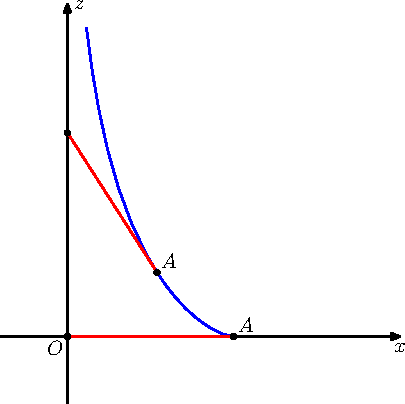
\includegraphics{tractrix}\\
      \captionof{figure}{拽物线}\label{fig:tractrix}\hfill
      \end{center}
      \begin{enumerate}\addtocounter{enumi}{15}
        \item 如图\ref{fig:tractrix}所示,
          我们将一个物体$A$用一根长为$1$的线拽着从原点出发沿着$z$轴正方向缓慢移动,
          $A$的运动轨迹称为\emph{拽物线}(tractrix). 它是以$z$轴为渐近线的光滑曲线.
          将拽物线沿着$z$轴旋转一周得到的旋转曲面称为\emph{拽物面}(tractricoid).
          将拽物面沿着$Oxy$-平面反射延拓得到的整个曲面称为\emph{伪球面}(pseudosphere),
          它是三维空间中具有常数高斯曲率$-1$的不完备非紧超曲面. 事实上,
          著名数学家Hilbert在1901年证明了不存在浸入到三维欧式空间且高斯曲率为负常数的正则完备曲面.
          关于伪球面的表面积与体积早在1693年由克里斯蒂安·惠更斯求出.
          他在1678年完成的《光论》(Trait\'e de la Lumi\`ere)中提出了关于波传播的著名的惠更斯原理.
          \begin{enumerate}
            \item 请首先证明拽物线$z=z(x)$满足常微分方程
              \begin{equation}\label{eq:tractrix}
                z'(x)=-\frac{\sqrt{1-x^2}}{x},\quad 0<x\leq 1.
              \end{equation}
              然后根据\eqref{eq:tractrix}验证拽物线可以参数化为
              \begin{equation}\label{eq:para-tractrix}
                x(t)=\sech t,\quad z(t)=t-\tanh t,\quad 0<t<+\infty.
              \end{equation}
              最后, 根据上述拽物线的参数方程写出拽物面的参数方程.

              回忆,
              \[
                \sech t=\frac{1}{\cosh t}=\frac{2}{e^{t}+e^{-t}},\quad\tanh t
                =\frac{\sinh t}{\cosh t}=\frac{e^{t}-e^{-t}}{e^{t}+e^{-t}}.
              \]
            \item 求拽物面$\Sigma$的表面积.
            \item 求拽物面和$Oxy$-平面围成的空间区域$\Omega$的体积.
          \end{enumerate}
          \vfill\null
          \columnbreak
          \begin{ans}[(a)]
            由图易知, 细线始终和$A$的轨迹相切. 假设$A=(x,z)$, 则$A$处的斜率直接计算得
            \[
              z'(x)=-\frac{\sqrt{1-x^2}}{x},\quad 0<x\leq1.
            \]
            这即表明拽物线$z=z(x)$满足常微分方程\eqref{eq:tractrix}. \dotfill{(4分)}

            由$z(t)=z(x(t))$, 利用复合函数求导知道
            \begin{align*}
              z'(t)&=z'(x)x'(t)=-\frac{\sqrt{1-[x(t)]^2}}{x(t)}\cdot x'(t)\\
                   &=-\sqrt{\cosh^2 t-1}\cdot \frac{-\sinh t}{\cosh^2t}
                   =\frac{\sinh^2 t}{\cosh^2t}=\tanh^2t.
            \end{align*}
            另一方面,
            \[
              z'(t)=1-\tanh't=1-\frac{1}{\cosh^2t}
              =\frac{\sinh^2 t}{\cosh^2t}=\tanh^2t.
            \]
            这表明, \eqref{eq:para-tractrix}确实满足微分方程\eqref{eq:tractrix}.
            \dotfill{(6分)}

            又由于$x(0)=1, z(0)=0$确实在拽物线上, 故由常微分方程的存在唯一性知
            \eqref{eq:para-tractrix}就是拽物线的参数化. \dotfill(8分)

            最后, 由拽物面是由拽物线$z=z(x)$绕着$z$轴旋转一周得到的. 故其参数方程为
            \[
              \begin{cases}
                x=\sech t\cos\theta,\\
                y=\sech t\sin\theta,\\
                z=t-\tanh t,
              \end{cases}\quad
              0\leq t<+\infty,\quad 0\leq \theta\leq 2\pi
            \tag{10分}
            \]
          \end{ans}

          \begin{ans}[(b)]
            我们可以将旋转面参数化为
            \[
              X(r,\theta)=\left(r\cos\theta,r\sin\theta,z(r)\right),
              0<r\leq1, 0\leq \theta\leq 2\pi,
            \]
            因此, 旋转曲面的面积微元为
            \[
              dS=\lvert X_r\times X_\theta \rvert drd\theta
              =r\sqrt{1+[z'(r)]^2}drd\theta,\tag{5分}
            \]
            因此, 旋转曲面的表面积为
            \[
              S=\int_0^{2\pi}d\theta\int_0^1 \lvert X_r\times X_\theta \rvert dr
              =2\pi\int_0^1r\sqrt{1+[z'(r)]^2}dr. \tag{8分}
            \]

            根据\eqref{eq:tractrix}, 我们得到
            \[
              \sqrt{1+z'^2(r)}=1/r,\implies S= 2\pi. \tag{10分}
            \]

            \textbf{法二}: 如果直接使用(a)中得到的参数方程
            \[
              X(t,\theta)=\left( \sech t\cos\theta,\sech t\sin\theta,t-\tanh t \right),
              \tag{2分}
            \]
            则容易算出
            \[
              dS=\lvert X_t\times X_\theta \rvert dt d\theta
              =\sech t\tanh t dt d\theta
              =\frac{\sinh t}{\cosh^2t} dt d\theta.\tag{5分}
            \]
            因此, $\Sigma$的表面积为
            \begin{align*}
              S&=\int_0^{2\pi}d\theta\int_0^{+\infty}\sech t\tanh tdt \tag{8分}\\
               &=-2\pi\int_0^{+\infty} d(\sech t)
                =2\pi.\tag{10分}
            \end{align*}
          \end{ans}

          \begin{ans}[(c)]
            使用\eqref{eq:para-tractrix}给出的参数化,
            \[
              X(t,\theta)=(\sech t\cos\theta,\sech t\sin\theta,t-\tanh t),\quad
              t\in[0,+\infty),\quad\theta\in[0,2\pi].
            \]
            因此,
            \[
              J=\frac{\partial(x,y)}{\partial(t,\theta)}=-\sech^2 t\tanh t.\tag{2分}
            \]
            故体积为
            \begin{align*}
              \lvert \Omega \rvert&=\iint_{x^2+y^2\leq 1}zdxdy
              =\int_0^{2\pi}d\theta\int_0^{+\infty}
              (t-\tanh t)\sech^2 t\tanh t dt,\tag{5分}\\
              \frac{\lvert \Omega \rvert}{2\pi}&=\int_0^1 (u\arctanh u-u^2) du,
              \quad(u=\tanh t, du=\sech^2 tdt)\\
              &=-\frac{1}{3}+\frac{1}{2}\int_0^1\arctanh u du^2\\
              &=-\frac{1}{3}+\frac{1}{2}\left( \left. u^2\arctanh u \right\rvert_{u=0}^1
              -\int_0^1 \frac{u^2}{1-u^2}du \right),\quad (\arctanh'u=\frac{1}{1-u^2})\\
              &=-\frac{1}{3}+\frac{1}{2}\left( \left. u^2\arctanh u \right\rvert_{u=0}^1
              +1-\frac{1}{2}\int_0^1\left( \frac{1}{1-u}+\frac{1}{1+u} \right)du \right)\\
              &=\frac{1}{6}+\frac{1}{2}\left. \left( u^2\arctanh u
              -\frac{1}{2}\left( -\ln(1-u)+\ln(1+u) \right) \right) \right\rvert_{u=0}^1\\
              &=\frac{1}{6}+\frac{1}{2}\lim_{u\to1^-}\left( u^2\arctanh u
              -\sqrt{\frac{1-u}{1+u}} \right).\tag{8分}
            \end{align*}
            将$u=\tanh t$, 代入
            \begin{align*}
              \lim_{u\to1^-}\left(u^2\arctanh u+\ln\sqrt{\frac{1-u}{1+u}}\right)
              &=\lim_{t\to+\infty}\left(t\tanh^2 t
              +\ln\sqrt{\frac{1-\tanh t}{1+\tanh t}}\right)\\
              &=\lim_{t\to+\infty}\left( t\frac{(e^{t}-e^{-t})}{e^{t}+e^{-t}}
              -\ln(\cosh t+\sinh t) \right)\\
              &=\lim_{t\to+\infty}(\frac{t(e^{t}-e^{-t})}{e^{t}+e^{-t}}-t)=0.
            \end{align*}
            因此
            \[
              \lvert \Omega \rvert=\pi/3.\tag{10分}
            \]
          \end{ans}
      \end{enumerate}
      \end{document}
%</maintex>
%    \end{macrocode}
%\CheckSum{0}
%\Finale
\endinput
